\documentclass[10pt,letterpaper,pdf]{article}
%%%%%%%%%%%%%%%%%%%%%%%%%%%%%%%%%%%%%%%%%%%%%%%%%%%%%%%%%%%%%%%%%
%% Adapted from <https://github.com/zachscrivena/simple-resume-cv>
%% and https://www.hansenlab.org/cv_bibliography_tex
%%%%%%%%%%%%%%%%%%%%%%%%%%%%%%%%%%%%%%%%%%%%%%%%%%%%%%%%%%%%%%%%%

%%%%%%%%%%%%%%%%%%%%%%%%%%%%%%%%%%%%%%%%%%%%%%%%%%%%%%%%%%%%%%%%%
%% PREAMBLE.
%%%%%%%%%%%%%%%%%%%%%%%%%%%%%%%%%%%%%%%%%%%%%%%%%%%%%%%%%%%%%%%%%
\usepackage{hyperref} % PDF settings and properties.
\usepackage[
  left=0.70in, right=0.70in, top=0.00in, bottom=0.45in, includehead, includefoot
  ]{geometry} % Geometry package for page margins.
% \usepackage{titlesec}
\usepackage[compact]{titlesec}
\usepackage[ampersand]{easylist}
\usepackage{tabularx}
\usepackage{fancyhdr}
\usepackage{lastpage}
\usepackage[utf8]{inputenc}
\usepackage[T1]{fontenc}
\usepackage[english]{babel}
\usepackage{csquotes}
\usepackage{color,hyperref,url}
\usepackage{graphicx,float}

% PDF settings and properties.
\definecolor{darkblue}{rgb}{0.0,0.25,0.0}
\hypersetup{
  bookmarksnumbered=false,
  pdftitle={Alex Gaudio},
  pdfauthor={Alex Gaudio Curriculum Vitae},
  pdfcreator={XeLaTeX},
  pdfproducer={},
  pdfkeywords={},
  unicode=true,
  bookmarksopen=true,
  pdfstartview=FitH,
  pdfpagelayout=OneColumn,
  pdfpagemode=UseOutlines,
  linktocpage=true,
  allcolors=darkblue,
  % urlcolor=darkblue,
  % linkcolor=darkblue,
  % citecolor=darkblue,
  % anchorcolor=darkblue,
  colorlinks,
  breaklinks
}
%
% Bibliography
% 
% \usepackage{biblatex}
\usepackage[backend=biber,
   bibstyle=numeric,sorting=ydnt,sortcites=true,natbib=true,defernumbers=true,
   maxbibnames=99,giveninits=true,uniquename=false]{biblatex}
\addbibresource{references.bib}
\renewcommand*{\mkbibnamegiven}[1]{
\ifitemannotation{highlight}
{\textbf{#1}}
{#1}}
\renewcommand*{\mkbibnamefamily}[1]{
\ifitemannotation{highlight}
  {\textbf{#1}}
  {#1}%
\ifitemannotation{first}
  {\textsuperscript{*}}
  {}%
\ifitemannotation{corresponding}
  {$^\dagger$}
  {}%
}%%

%
% Page settings
%
\pagestyle{plain}
% Paragraph style.
\setlength{\parindent}{0in} % No indentation at the beginning of each paragraph.
\setlength{\parskip}{0in} % No vertical space between paragraphs.
% Avoid bad page breaks within paragraphs.
\widowpenalties 1 10000
\clubpenalties 1 10000
\raggedbottom
% Avoid overfull lines.
\sloppy
%
% Formatting details
%
\newcommand{\DatestampYM}[2]{\mbox{\ShortMonth{#2} #1}}
\newcommand{\DatestampY}[1]{\mbox{ #1}}
\newcommand{\LongMonth}[1]{%
\ifcase#1\relax
\or January%
\or February%
\or March%
\or April%
\or May%
\or June%
\or July%
\or August%
\or September%
\or October%
\or November%
\or December%
\fi}
\newcommand{\ShortMonth}[1]{%
\ifcase#1\relax
\or Jan%
\or Feb%
\or Mar%
\or Apr%
\or May%
\or Jun%
\or Jul%
\or Aug%
\or Sep%
\or Oct%
\or Nov%
\or Dec%
\fi}

\newcommand{\BulletSymbol}{{\normalfont\fontsize{6.5}{7.8}\selectfont\raisebox{0.17em}{\char"25A0}}}
\newcommand{\SubBulletSymbol}{{\normalfont\fontsize{6}{7.2}\selectfont\raisebox{0.17em}{\char"25CF}}}

% Section numbering disabled:
% we use \prefix@<level> only if it is defined
\makeatletter
\renewcommand{\@seccntformat}[1]{%
  \ifcsname prefix@#1\endcsname
    \csname prefix@#1\endcsname
  \else
    \csname the#1\endcsname\quad
  \fi}
\newcommand\prefix@section{}
\newcommand\prefix@subsection{}
\makeatother

% \HUGE font size
\makeatletter
\newcommand\HUGE{\@setfontsize\Huge{40}{50}}
\makeatother

\title{
\begin{minipage}{1.5cm}
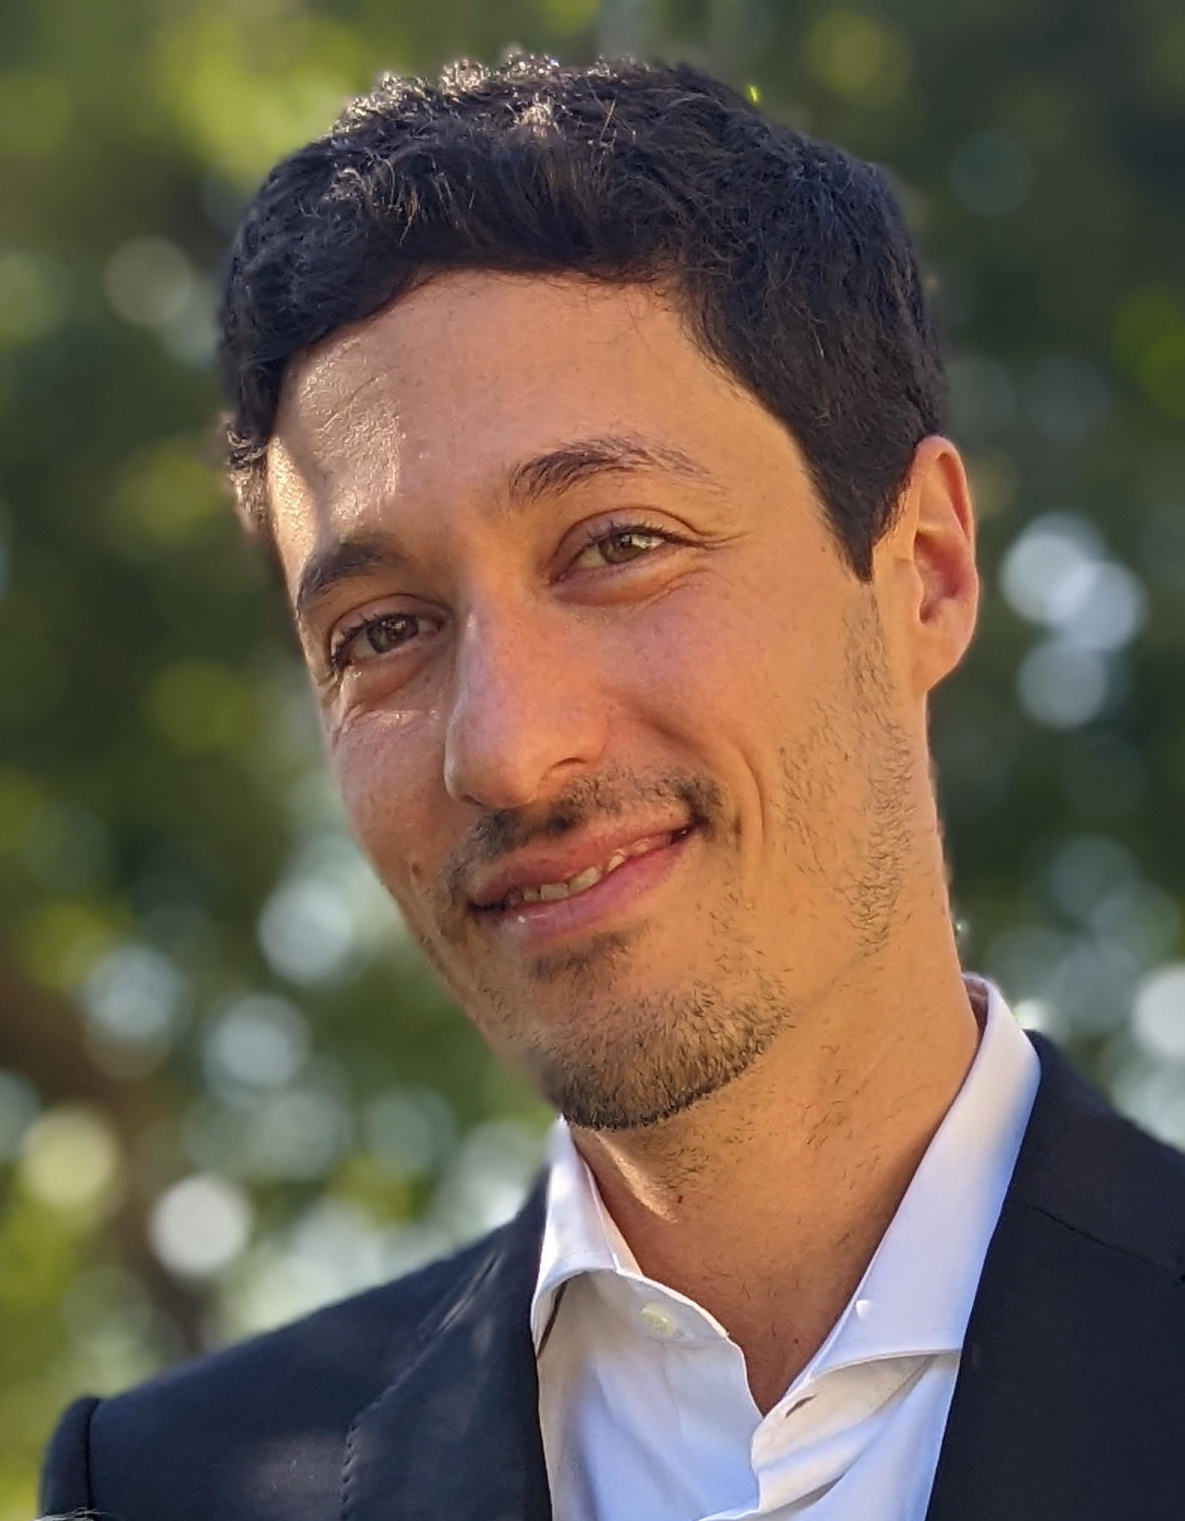
\includegraphics[width=\linewidth]{profile_pic.jpg}
\end{minipage}
\quad
\begin{tabular}{l}
\HUGE\textbf{Alex Gaudio}
\end{tabular}
\hfill
% \large \raggedleft
\large
\begingroup
\hfill
\begin{tabularx}{7.2cm}{l l}
  Email:   &\href{mailto:adgaudio@gmail.com}{adgaudio@gmail.com}\\
  Website: &\href{http://www.alexgaudio.com}{alexgaudio.com}\\
  GitHub:  &\href{https://www.github.com/adgaudio}{github.com/adgaudio}\\
  LinkedIn:&\href{https://www.linkedin.com/in/adgaudio}{linkedin.com/in/adgaudio}\\
\end{tabularx}
\endgroup
\vspace{-1.5cm}
}
\date{}
\author{}

% \makeatletter
% \makeatother

% formatting
\titleformat{\section}{\Large\bfseries\uppercase}{}{0pt}{}
% \titleformat*{\section}{\Large\bfseries\uppercase}
% \titlespacing{\section}{0pt}{*4}{*1.5}
\titlespacing\section{0pt}{12pt plus 4pt minus 2pt}{0pt plus 2pt minus 2pt}
\titleformat*{\subsection}{\large\bfseries}
% page numbering
\pagestyle{fancy} % Turn on the style
\fancyhf{} % Start with clearing everything in the header and footer
\fancyfoot[C]{Alex Gaudio -- \thepage\ of \pageref{LastPage}}

% \tracingmacros=1 
\begin{document}
% \tracingmacros=0 
\maketitle

\vbox{
  \section{Education}

  \subsection{\href{http://www.cmu.edu}{\textbf{Carnegie Mellon University}}}
  \ \ \textbf{Ph.D. Candidate in Electrical Computer Engineering}
  \hfill
  \textbf{\DatestampYM{2018}{08} -- current }
  \ \ \begin{easylist}[itemize] \ListProperties(Space=0em, Space*=0em)
    & Advisors: Professor Asim Smailagic and Professor Aur{\'e}lio Campilho
    & Thesis: Explainable Deep and Machine Learning for Medical Image Analysis
  \end{easylist}

  \subsection{\href{https://sigarra.up.pt/feup/en/web_page.inicial}{\textbf{University of Porto, Faculdade de Engenharia}}}
  \ \ \textbf{Ph.D. Candidate in Electrical Computer Engineering}
  \hfill
  \textbf{\DatestampYM{2018}{08} -- current }
  \ \ \begin{easylist}[itemize] \ListProperties(Space=0em, Space*=0em)
          & Advisors: Professor Aur{\'e}lio Campilho and Professor Asim Smailagic
    & Fellowship awarded through the \href{https://www.cmuportugal.org/}{CMU Portugal Program} for Dual Ph.D. Degrees
  \end{easylist}

  \subsection{\href{https://www.cmu.edu}{\textbf{Carnegie Mellon University}}}
  \ \ \textbf{Masters in Electrical Computer Engineering}
  \hfill
  \textbf{\DatestampYM{2018}{08} -- current }
  \ \ \begin{easylist}[itemize] \ListProperties(Space=0em, Space*=0em)
          & Advisors: Professor Asim Smailagic and Professor Aur{\'e}lio Campilho
  \end{easylist}

  \subsection{\href{https://www.bard.edu}{\textbf{Bard College}}}
  \ \ \textbf{Bachelor of Arts in Music}
  \hfill
  \textbf{\DatestampYM{2006}{08} -- \DatestampYM{2010}{05}}
  \ \ \begin{easylist}[itemize] \ListProperties(Space=0em, Space*=0em)
    & Award: Recipient of the Larry McLeod Award in Jazz.
    & Thesis: Connecting With Others Through Jazz: Performances and All-Original Composition
  \end{easylist}
}

\nocite{*}

\defbibnote{mynote}{\qquad$^*$ indicates equal contributions\qquad $^\dagger$ indicates corresponding author(s)}
   % \\ \textbf{boldface} indicates a member of my lab \\}
\printbibliography[keyword={journal}, title={Journal Publications (Peer-Reviewed) }, prenote=mynote]
\printbibliography[keyword={conference}, title={Conference Publications (Peer-Reviewed)}]
\printbibliography[keyword={patent}, title={Patents}]
\printbibliography[keyword={invitedtalk}, title={Invited Talks}]

\section{Teaching}
% TODO: Teaching also in references.bib
\subsection{\small Fall 2021, Intro to Machine Learning (PhD Level), Teaching Assistant}
\begin{easylist} \ListProperties(Space=0em, Space*=0em)
    & With Prof. Jaime Cardoso at FEUP, University of Porto, Portugal
    & Three lectures, each three hours long, and weekly office hours. \href{https://docs.google.com/presentation/d/1joBU3QM3jcpMYBDeFdvwiuDHdXrLZweiAiW1BgXMN7E/edit?usp=sharing}{slides1} \href{https://docs.google.com/presentation/d/1OkectcY5ImaDDD-a2M4ZRNoKgxxkM5DyoJ3oRK_vKn8/edit?usp=sharing}{slides2} \href{https://docs.google.com/presentation/d/14uhYMDF_xdyQosnJnFvr8sqUh31SGAtaN7V4Ob6f13Q/edit?usp=sharing}{slides3}
\end{easylist}

\subsection{\small Spring 2022, Intro to Biomedical Engineering (Undergraduate
Level), Teaching Assistant}
\begin{easylist} \ListProperties(Space=0em, Space*=0em)
    & With Prof. Ana Maria Mendon{\,c}a at FEUP, University of Porto, Portugal
    & Two lectures, each one hour long.  \href{https://docs.google.com/presentation/d/1lco5nlckinGk8RVHosJapeGzfjR6MUC9TbwOuRjUSms/edit?usp=sharing}{slides}
\end{easylist}

% \printbibliography[keyword={teaching}, category={teaching}]

\section{Industry Experience}
% columbia
\subsection{\small\href{http://www.nycmakerspace.org/}{NYC Makerspace}: Co-Founder
\DatestampYM{2017}{02} -- \DatestampYM{2020}{10} }
\begin{easylist}[itemize] \ListProperties(Space=0em, Space*=0em)
  & A non-profit establishing makerspaces
  throughout New York City.  We provide advanced resources and
  education freely to the public, where learning and
  innovation is a form of recreation.
  & Forged partnerships with Columbia University, Columbia Teacher's College and NYC Parks and
  Recreation.
  & Taught three 12-week courses on robotics, programming, mathematics and 3D modeling to high school seniors.
  & Established Harlem's first makerspace, and brought over \$17,000 to the space.
  & Honored as a Champion of Social Justice by the Wilson Major Morris Community Center in Jan. 2018.
\end{easylist}

\subsection{\small\href{http://www.creativemachineslab.com/}{Columbia University, Creative Machines Lab (Prof. Hod Lipson)}
%\hfill \DatestampYM{2016}{12} -- \DatestampYM{2018}{06}}
}
\begin{easylist}[itemize] \ListProperties(Space=0em, Space*=0em)
  & \textbf{Software Engineer: DARPA Transformative Design (TRADES) program
\hfill \DatestampYM{2017}{11} -- \DatestampYM{2018}{06}}
&& Mass-spring simulator for generative design of 3D models, an alternative to Finite Element Analysis.
& \textbf{Independent Research, advised by Prof. Hod Lipson
  \hfill \DatestampYM{2016}{12} -- \DatestampYM{2017}{07}}
  && Multi-Agent Collaborative Learning simulator: \href{http://www.github.com/adgaudio/MACL}{MACL}.
\end{easylist}

\subsection{\small\href{http://buildinglink.com/}{BuildingLink}: Data Scientist
\DatestampYM{2016}{11} -- \DatestampYM{2018}{07}}
\begin{easylist}[itemize] \ListProperties(Space=0em, Space*=0em)
  & \href{https://vimeo.com/234396442}{ImageR}: Machine Learning and Vision to solve matching problems, such as to connect images of packages to building residents.
  I designed and implemented the production ready algorithms, then coordinated development and release of the mobile apps for iOS and Android.
  ImageR processes 50K packages a day, 18 million packages processed by Jan. 2021, launched May 2018.  Awarded Patent: 10,803,542 
\end{easylist}

\subsection{\small\href{http://www.alluvium.io}{\textbf{Alluvium}}: Senior Data Scientist, 1st employee
\DatestampYM{2015}{12} -- \DatestampYM{2016}{05}}
\begin{easylist}[itemize] \ListProperties(Space=0em, Space*=0em)
  & Machine learning and IoT business that deploys
  intelligent autonomous agents close to sources of streaming
  data.
\end{easylist}

\subsection{\small\href{http://www.sailthru.com}{\textbf{Sailthru}}: Senior Data Scientist and Engineer
\DatestampYM{2012}{08} -- \DatestampYM{2015}{11}}
\begin{easylist}[itemize] \ListProperties(Space=0em, Space*=0em)
  & Inc. 5000’s $30^{th}$ fastest-growing company in the US in 2013.  Subsequently acquired in 2019.
  & Founded data science team, hired my boss, VP of
  Data Science Jeremy Stanley and grew team from 1 to 4 full
  time employees. Promotion to "Senior" in 2014.
  & Created and launched \href{https://www.businesswire.com/news/home/20141029005714/en/Sailthru-Announces-Sailthru-Sightlines-Bringing-Accurate-and-Automated-Consumer-Predictions-To-Ecommerce-and-Media-Brands}{Sightlines\textsuperscript{TM}} to predict user behavior, and architected a robust, fault tolerant and distributed data science platform.
\end{easylist}

\subsection{\small\href{http://www.adaptly.com}{\textbf{Adaptly}}: Developer
\DatestampYM{2011}{12} -- \DatestampYM{2012}{07}}
% \begin{easylist}[itemize] \ListProperties(Space=0em, Space*=0em)
%   & Data science and big data engineering for Facebook advertising, subsequently acquired in 2018.
% \end{easylist}

\vbox{\subsection{\small\href{http://www.flatworldknowledge.com}{\textbf{Flat World Knowledge}}: Software Engineer, Backend
\DatestampYM{2011}{02} -- \DatestampYM{2011}{12}}
% \begin{easylist}
%   & Automated textbook publishing platform to produce low-cost, customizable
%   textbooks for classrooms.
% \end{easylist}
}

\vbox{\subsection{\small\href{http://www.bard.edu/}{Bard College}: Systems Engineer
\DatestampYM{2009}{07} -- \DatestampYM{2010}{09}}
% \begin{easylist}
%   & Supervised by CTO Bill Terry. Collaborated with REN-ISAC (Research \& Education Networking Information Sharing \& Analysis Center).
% \end{easylist}
}

\vbox{\subsection{\small\href{https://www.lmhospital.org/}{Lawrence and Memorial Hospital}:
Emergency Room Technician (Level I)
\DatestampYM{2008}{06} -- \DatestampYM{2008}{08}}
% \begin{easylist}
%   & Summer job during college.
% \end{easylist}
}
\vbox{\subsection{\small\href{https://www.ndpems.com/}{NDP Emergency Medical Services}:
Emergency Medical Technician (EMT-B)
\DatestampYM{2007}{11} -- \DatestampYM{2008}{03}}
% \begin{easylist}
%   & Side job during college.
% \end{easylist}
}


% \section{Open Source Projects}
% \ \  Projects for which I am the sole contributor\\ \\
% \begin{tabularx}{\textwidth}{l X}
  % \href{https://www.github.com/adgaudio/MACL}{MACL} & Simulator to study multi-agent learning in N-dimensional environments.
  % \\
  % \href{https://www.github.com/sailthru/stolos}{Stolos} & A distributed task dependency scheduler designed to simplify complex distributed pipelines.
  % \\
  % \href{https://www.github.com/sailthru/relay}{Relay} & Self-tuning PID algorithm
  % that minimizes the difference of two eventually consistent timeseries.
  % \\
  % \href{https://www.github.com/sailthru/relay.mesos}{Relay.Mesos} & Autoscale tasks on Mesos using the Relay algorithm.
  % \\
  % \href{https://www.github.com/adgaudio/MajorityRedis}{MajorityRedis} &
  % Redis client using quorum of Redis instances to get strong consistency and partition tolerance.
  % \\
  % \href{https://github.com/adgaudio/dlp_printer}{dlp\_printer} & Designs of a DLP Stereolithography printer built from scratch.
% \end{tabularx}


\section{Awards}
\begin{easylist}
    & \textbf{Dual PhD Degree Fellowship} from Carnegie Mellon University, Portugal Program \hfill \DatestampYM{2018}{08}
    & \textbf{Champion of Social Justice} from the Wilson Major Morris Community
    Center in Harlem, NY \hfill \DatestampYM{2018}{01}
    & \textbf{Larry McLeod Award in Jazz} from Bard College \hfill \DatestampYM{2010}{05}
\end{easylist}
% \\
% \textbf{Honored as Champion of Social Justice by the Wilson Major Morris Community Center.} \hfill \DatestampYM{2018}{01}
% \\
% \textbf{Sailthru Robotics Hackathon Competition.}  1st place, won \$100. \hfill \DatestampYM{2014}{06}
% \\
% \textbf{Kaggle Data Science Competition.} \href{https://www.kaggle.com/c/dsg-hackathon/leaderboard}{5th place in NY and 28th globally.} \hfill \DatestampYM{2012}{04}
% \\
% \textbf{Coursera Machine Learning Course.} \href{http://alexgaudio.com/img/ml_statement_of_accomplishment.pdf}{Perfect score in course.} \hfill \DatestampYM{2011}{12}
% \\
% \textbf{Recipient of the Larry McLeod Award in Jazz.} \hfill \DatestampYM{2010}{05}


\end{document}
